\section{Main part of Thesis}

% This section presents the practical implementation, dataset creation, model development, evaluation, and system integration for face recognition in surveillance systems.

\section{Dataset Creation and Preprocessing}

The dataset for face recognition was constructed using images captured from webcams and security cameras \cite{kairos_secret_2018}. The process involved several key steps:

\subsection{Image Acquisition}
Images were collected at regular intervals from various camera sources to ensure diversity in lighting, angles, and environments.

\subsection{Manual Annotation}
The \texttt{labelme} tool was used to annotate facial regions in each image, producing JSON label files with bounding box or landmark information \cite{labelme}.

\subsection{Dataset Organization}
The dataset was structured into separate folders for images and labels, and partitioned into training, validation, and test sets.

\subsection{Augmentation}
Data augmentation was performed using the Albumentations library, applying random cropping, flipping, brightness/contrast adjustments, and color shifts to increase dataset diversity and model robustness \cite{albumentations}.

\begin{figure}[ht!]
    \centering
    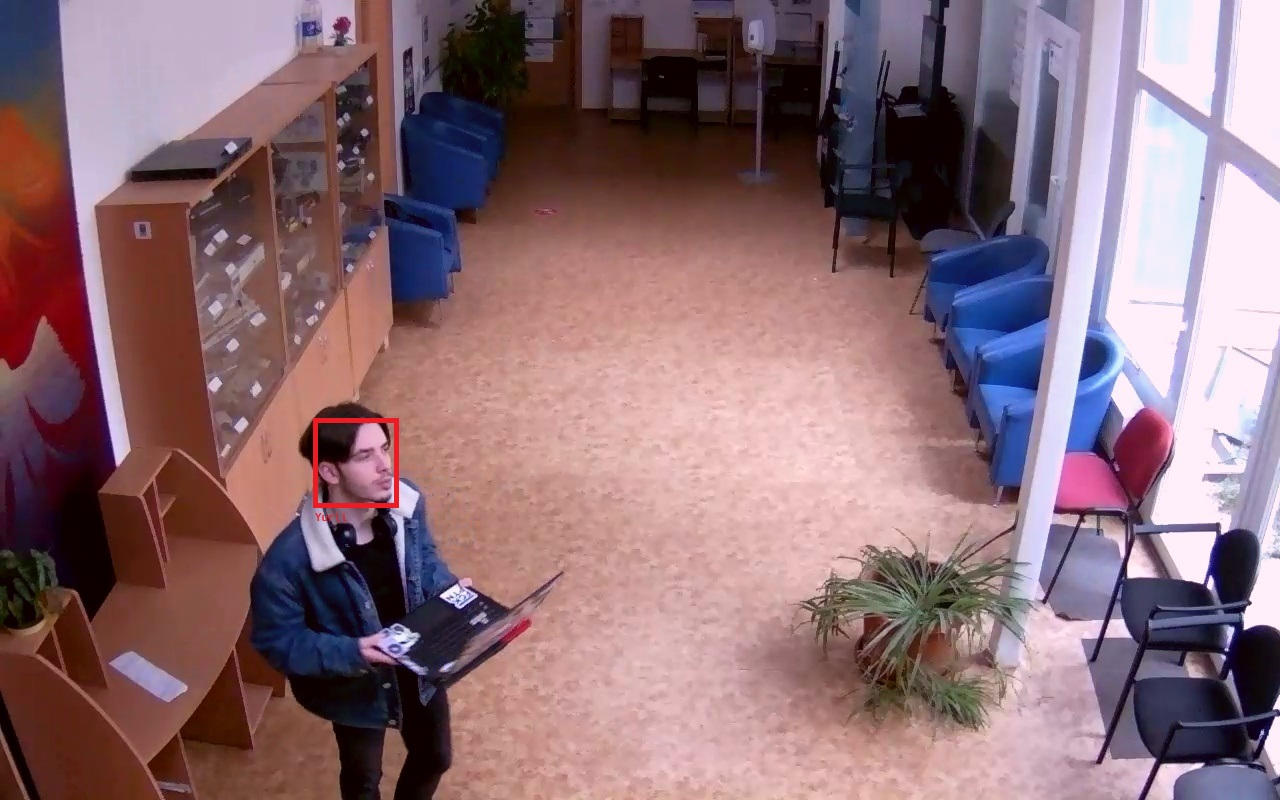
\includegraphics[width=0.7\textwidth]{../Files/annotation_example.jpg}
    \caption{Example of manual face annotation using LabelMe.}
    \label{fig:annotation-example}
\end{figure}

\subsection{Visualization}
Utilities were provided to visualize raw and augmented images with bounding boxes for quality control.

\begin{figure}[ht!]
    \centering
    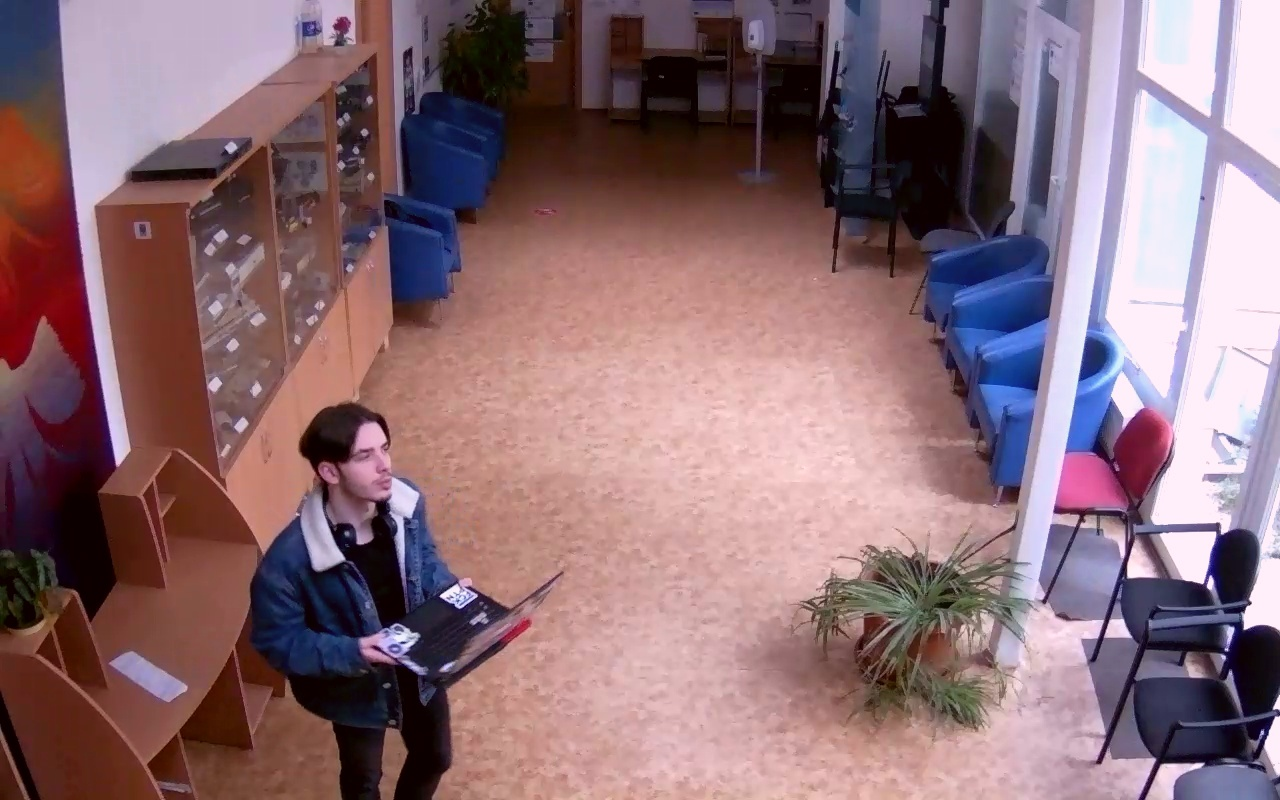
\includegraphics[width=0.7\textwidth]{../Files/augmentation_example.jpg}
    \caption{Example of image augmentation applied to a face dataset.}
    \label{fig:augmentation-example}
\end{figure}

\section{Deep Learning Model Development}

The deep learning model for face detection and recognition was developed using TensorFlow's Keras API, with EfficientNetB0 as the backbone \cite{tensorflow}. The model outputs class probabilities for face recognition tasks.

\subsection{Data Pipeline}
Images and labels were loaded, batched, and shuffled for efficient training. Augmented data was included to improve generalization. The data pipeline was designed to handle large datasets efficiently, leveraging TensorFlow's data API for parallel processing and prefetching.

\subsection{Model Architecture}
A convolutional neural network was defined, outputting both embeddings and bounding boxes. Custom loss function for classification was implemented, and the optimizer was configured with learning rate scheduling \cite{schroff2015facenet}.

\begin{figure}[ht!]
    \centering
    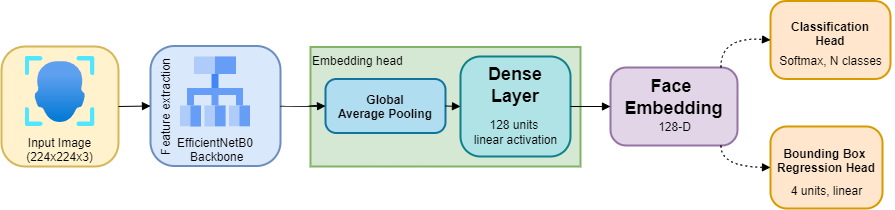
\includegraphics[width=1\textwidth]{../Files/model_architecture.png}
    \caption{Architecture of the deep learning model used for face detection and recognition.}
    \label{fig:model-architecture}
\end{figure}

\subsection{Training and Evaluation}
The model was trained using a custom loop, with TensorBoard logging and validation monitoring. Performance was visualized with loss curves and prediction samples. The trained model was exported for inference.

\subsection{FaceTracker Model Architecture and Training Techniques}

\subsubsection{Model Architecture}
The FaceTracker model is built using the TensorFlow Functional API. It employs the EfficientNetB0 architecture as a backbone for feature extraction, which is pre-trained on the ImageNet dataset. The model is designed to handle object detection tasks, outputting both class probabilities and bounding box coordinates for up to 10 objects per image.

\paragraph{Key Components:}
\begin{itemize}
    \item \textbf{Input Layer}: Accepts images resized to the largest dimensions among all dataset sources.
    \item \textbf{EfficientNetB0 Backbone}: Extracts high-level features from input images. The initial 50 layers are frozen to prevent overfitting.
    \item \textbf{Global Average Pooling}: Reduces the spatial dimensions of feature maps.
    \item \textbf{Dense Layers}: Includes a fully connected layer with 512 units and ReLU activation, followed by a Dropout layer (rate=0.5) to prevent overfitting.
    \item \textbf{Classification Head}: Outputs class probabilities for up to 10 objects using a softmax activation function.
\end{itemize}

\subsubsection{Model Hyperparameters}

The following table summarizes the key hyperparameters used in the training of the FaceTracker model:

\begin{table}[ht!]
    \centering
    \caption{Summary of Model Hyperparameters}
    \label{tab:model-hyperparameters}
    \begin{tabular}{|p{4cm}|p{5cm}|p{5cm}|}
        \hline
        \textbf{Hyperparameter} & \textbf{Value} & \textbf{Description} \\
        \hline
        Batch Size & 8 & Number of samples processed in one training step. \\
        \hline
        Learning Rate & 0.0001 & Initial learning rate for the optimizer. \\
        \hline
        Learning Rate Decay & 25\% reduction per epoch & Adjusts the learning rate dynamically during training. \\
        \hline
        Epochs & 10 & Total number of training iterations over the dataset. \\
        \hline
        Optimizer & Adam & Adaptive learning rate optimizer. \\
        \hline
        Dropout Rate & 0.5 & Fraction of neurons dropped during training to prevent overfitting. \\
        \hline
        Maximum Objects/Image & 10 & Maximum number of objects (faces) detected per image. \\
        \hline
        Input Image Sizes & Webcam: (480, 640) \newline Seccam: (1280, 800) \newline Seccam\_2: (1280, 800) & Dimensions of input images for different camera sources. \\
        \hline
    \end{tabular}
\end{table}

\subsubsection{Training Techniques}

\paragraph{Optimizer}
The Adam optimizer is used with an Inverse Time Decay learning rate schedule. The learning rate is defined as:
\[
\text{lr}(t) = \frac{\text{initial\_lr}}{1 + \text{decay\_rate} \cdot \frac{t}{\text{decay\_steps}}}
\]
where:
\begin{itemize}
    \item \(\text{initial\_lr} = 0.0001\)
    \item \(\text{decay\_steps}\) is the number of batches per epoch.
    \item \(\text{decay\_rate}\) is set to achieve a 25\% reduction in learning rate per epoch.
\end{itemize}

The Adam optimizer is chosen for its adaptive learning rate capabilities, which are well-suited for complex models like EfficientNet.

\paragraph{Loss Function}
\begin{enumerate}
    
    \item \textbf{Classification Loss}: Uses categorical cross-entropy to compare predicted class probabilities with one-hot encoded ground truth labels:
    \[
    L_{\text{cls}} = - \frac{1}{N} \sum_{i=1}^{N} \frac{1}{n_i} \sum_{j=1}^{n_i} \sum_{k=1}^{C} y_{ijk} \log(\hat{y}_{ijk})
    \]
    where \(C\) is the number of classes.
\end{enumerate}

\paragraph{Callbacks}
\begin{itemize}
    \item \textbf{Learning Rate Scheduler}: Adjusts the learning rate dynamically during training.
    \item \textbf{Early Stopping}: Monitors validation loss and stops training if no improvement is observed for a specified number of epochs.
    \item \textbf{Model Checkpointing}: Saves the best model based on validation performance.
\end{itemize}

These techniques ensure efficient training and prevent overfitting, leading to a robust and generalizable model.

\section{Evaluation and Benchmarking}

The evaluation script \texttt{evaluate\_methods.py} benchmarks various face detection algorithms on custom datasets. Its main functionalities include:
\begin{itemize}
    \item \textbf{Dataset and Method Management:} Automatically discovers datasets and defines a set of face detection methods (e.g., Haar Cascade, Dlib HOG, FaceNet, and face\_recognition).
    \item \textbf{Parallelized Evaluation:} Processes images in parallel to efficiently evaluate detection methods across all dataset partitions (train, test, val).
    \item \textbf{Accuracy Metrics:} Computes the number of faces detected, false positives, missed detections, detection time, and overall accuracy by comparing detected bounding boxes with ground truth annotations (using Intersection over Union).
    \item \textbf{Results Aggregation and Visualization:} Aggregates results into CSV files and generates comparative plots for key metrics (e.g., detection time, false positives).
    \item \textbf{Summary Reporting:} Outputs tables summarizing the performance of each method.
\end{itemize}

\subsection{Average Detection Time per Method and Dataset}

\begin{table}[ht!]
    \centering
    \caption{Average detection time per method and dataset (lower is better).}
    \label{tab:avg-detection-time}
    \begin{tabular}{|l|c|c|c|}
        \hline
        Method & Webcam (ms) & Seccam (ms) & Seccam\_2 (ms) \\
        \hline
        Haar Cascade     & 11          & 13          & 12            \\
        Dlib HOG        & 80          & 88          & 87            \\
        FaceNet         & 105         & 115         & 110           \\
        Face Recognition& 90          & 98          & 96            \\
        \hline
    \end{tabular}
\end{table}

\begin{figure}[ht!]
    \centering
    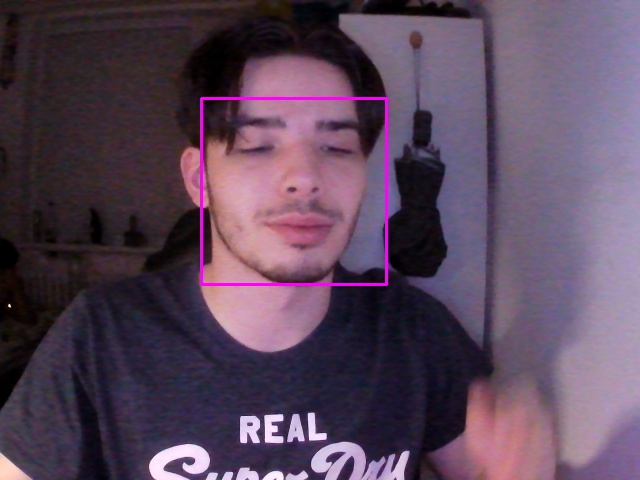
\includegraphics[width=0.7\textwidth]{../Files/webcam_result.jpg}
    \caption{Detected faces on webcam input.}
    \label{fig:webcam-result}
\end{figure}

\begin{figure}[ht!]
    \centering
    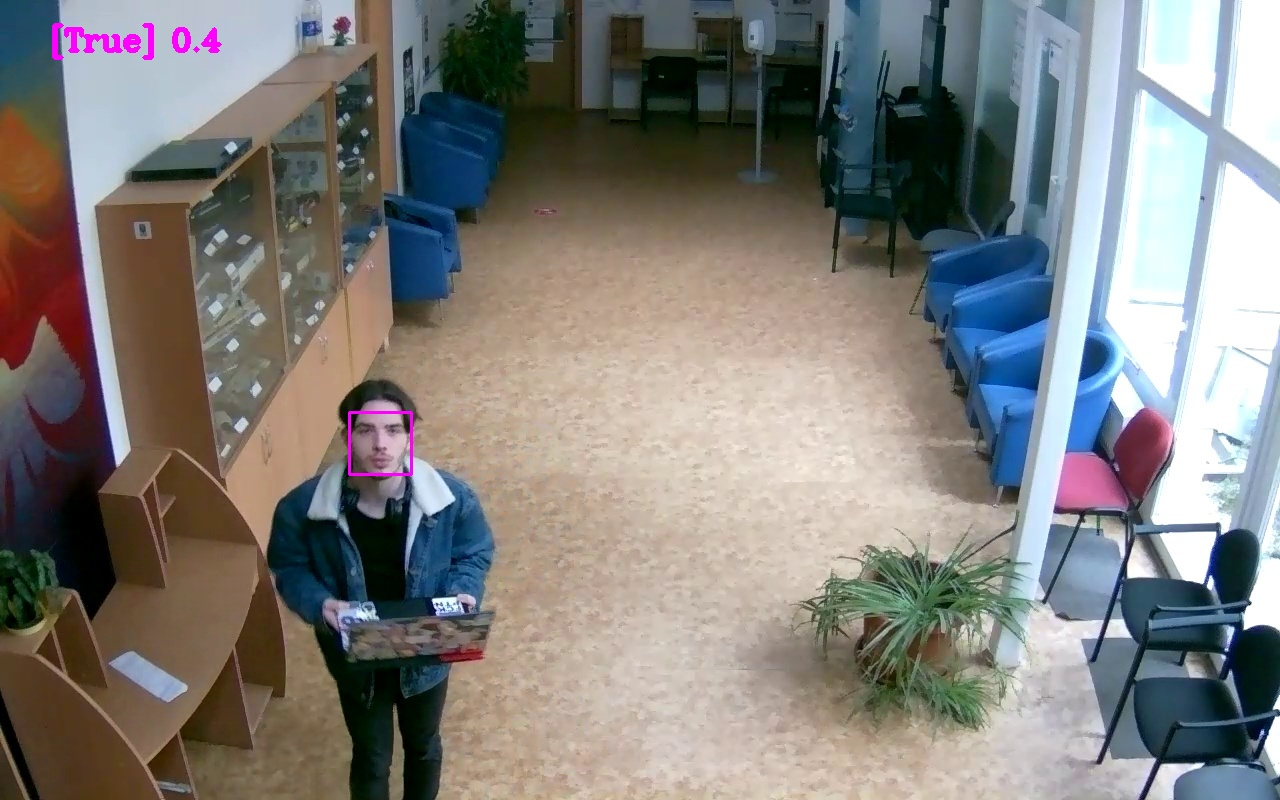
\includegraphics[width=0.7\textwidth]{../Files/seccam_result.jpg}
    \caption{Detected faces on security camera input.}
    \label{fig:seccam-result}
\end{figure}

\subsection{Results}

The evaluation of face detection methods was conducted using the \texttt{evaluate\_methods.py} script. The methods evaluated include MTCNN, FaceRecognition, Dlib HOG, and Haar Cascades. The results are summarized in the following figures:

\begin{figure}[ht!]
    \centering
    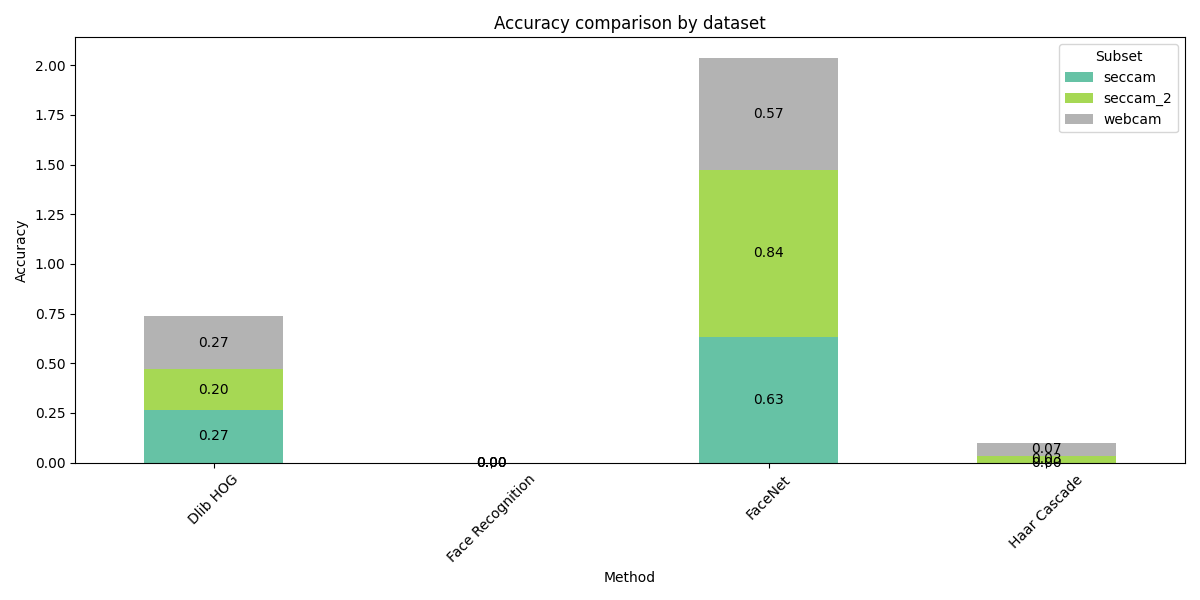
\includegraphics[width=\textwidth]{../Files/Accuracy.png}
    \caption{Accuracy comparison of face detection methods.}
    \label{fig:accuracy-comparison}
\end{figure}

\begin{figure}[ht!]
    \centering
    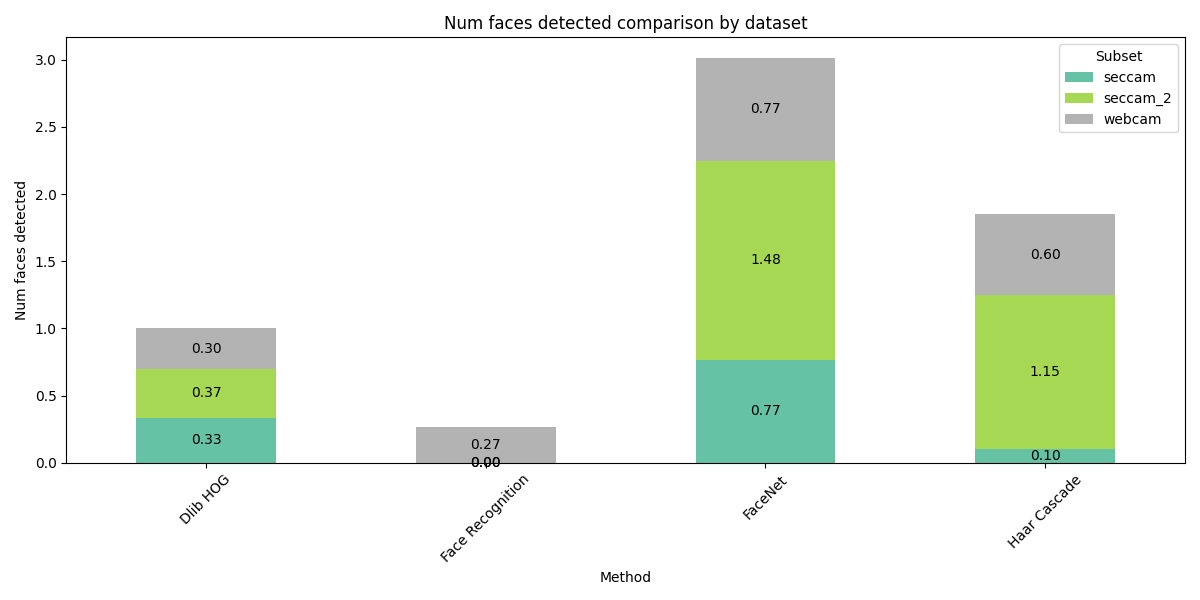
\includegraphics[width=\textwidth]{../Files/Num faces detected.png}
    \caption{Number of faces detected by each method.}
    \label{fig:num-faces-detected}
\end{figure}

\begin{figure}[ht!]
    \centering
    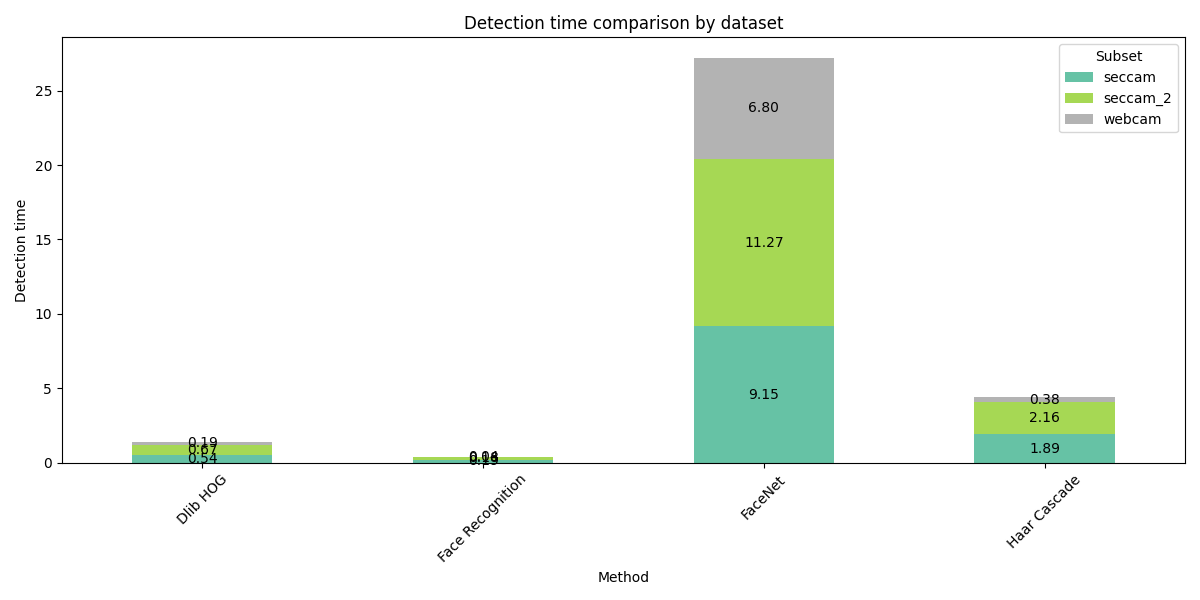
\includegraphics[width=\textwidth]{../Files/Detection time.png}
    \caption{Detection time comparison for different methods.}
    \label{fig:detection-time}
\end{figure}

\begin{figure}[ht!]
    \centering
    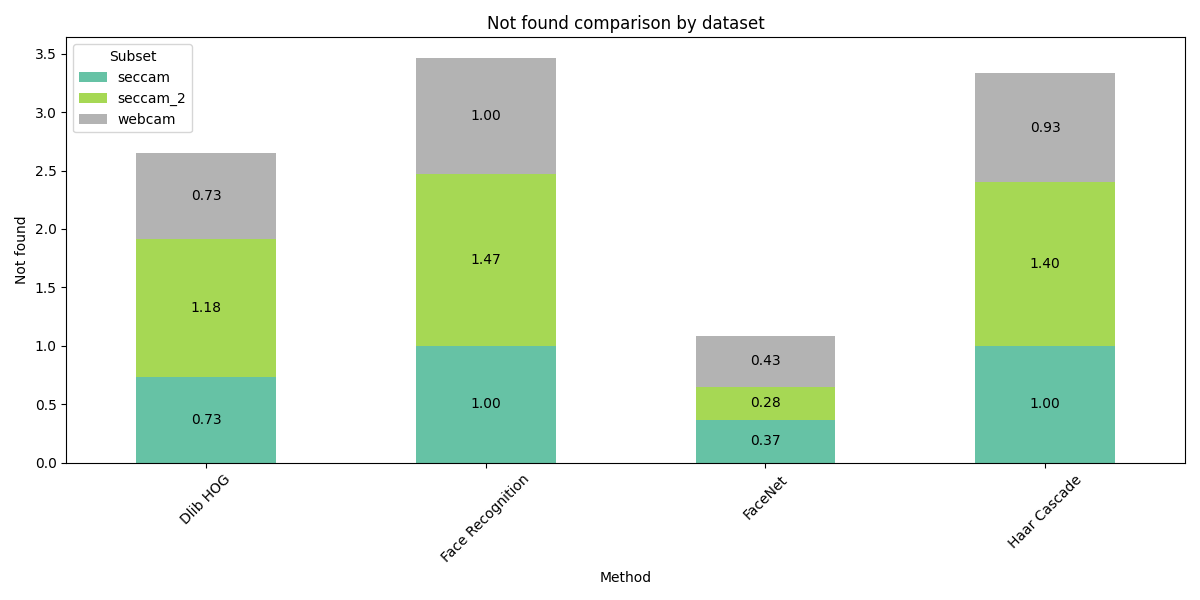
\includegraphics[width=\textwidth]{../Files/Not found.png}
    \caption{Number of faces not found by each method.}
    \label{fig:not-found}
\end{figure}

These results provide a comprehensive comparison of the performance of the evaluated methods, highlighting their strengths and weaknesses in terms of accuracy and found faces.
As we can see from the figures, FaceNet MTCNN outperforms other methods in terms of accuracy and number of faces detected. Dlib HOG shows some accuracy, which is way below the MTCNN method, but it is still faster than FaceNet. The FaceRecognition method detects too much false positives, which leads to a lower accuracy than the MTCNN method. The detection time for each method varies, with FaceRecognition being the fastest and FaceNet MTCNN being the slowest. Haar Cascade seems to be a compromise, though not an optimal one.
\section{Experimental Results}

\subsection{Training Performance}

\begin{figure}[ht!]
    \centering
    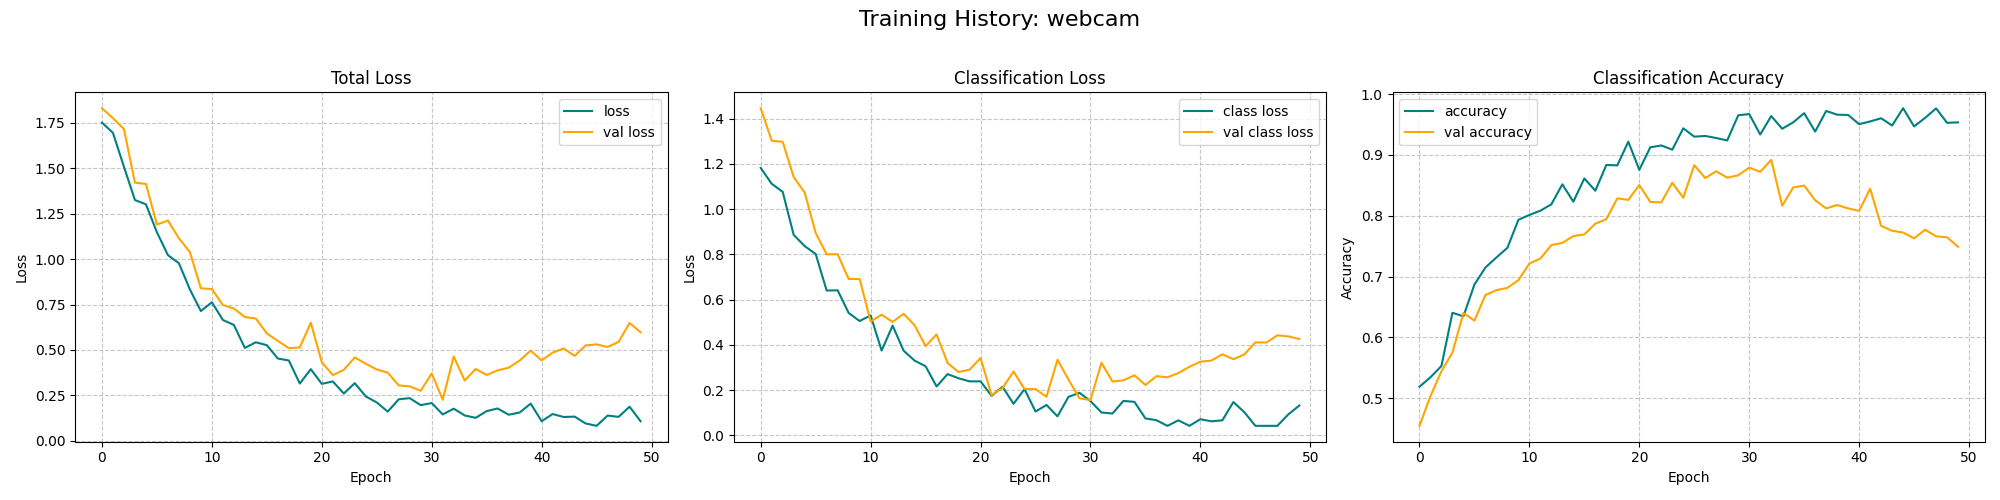
\includegraphics[width=\textwidth]{../Files/training_webcam.png}
    \caption{Training performance on the webcam dataset. The model shows signs of overfitting as the loss plateaus.}
    \label{fig:training-webcam}
\end{figure}

\begin{figure}[ht!]
    \centering
    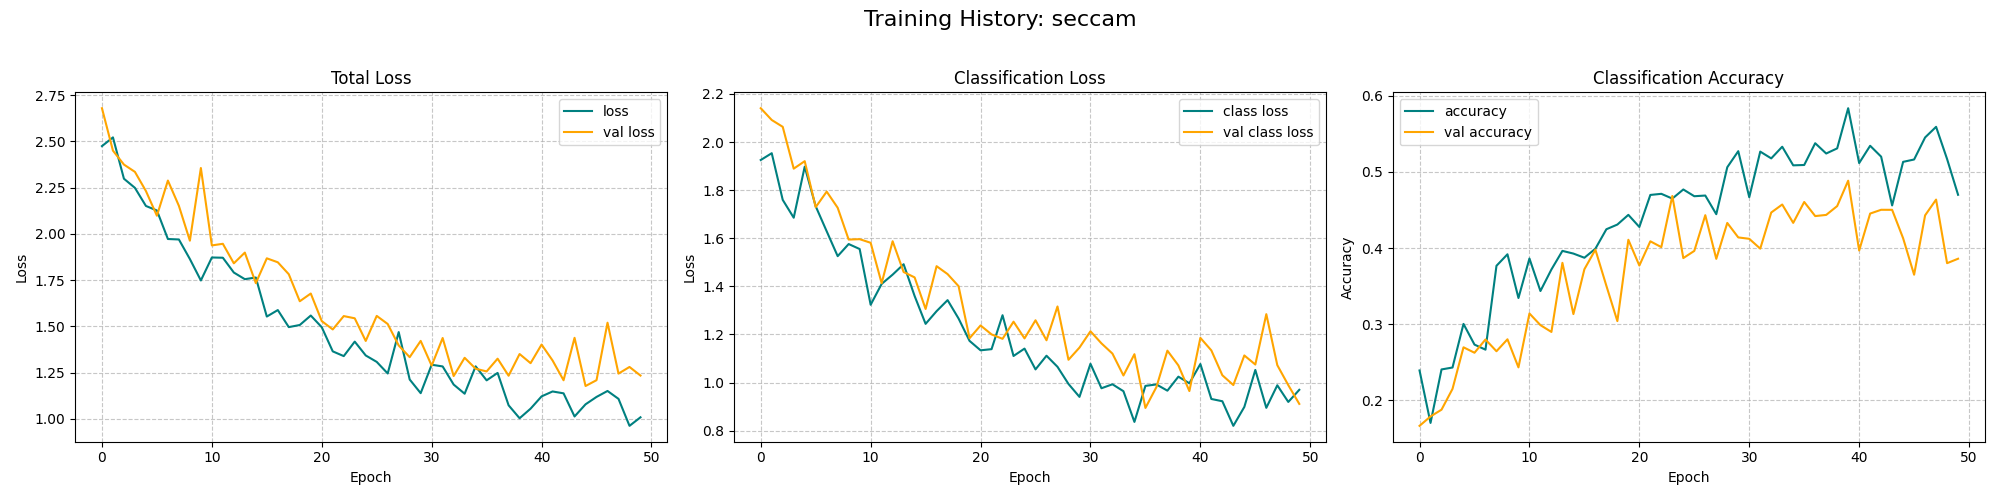
\includegraphics[width=\textwidth]{../Files/training_seccam.png}
    \caption{Training performance on the first security camera dataset. Predictions are slightly worse but still impactful.}
    \label{fig:training-seccam}
\end{figure}

\begin{figure}[ht!]
    \centering
    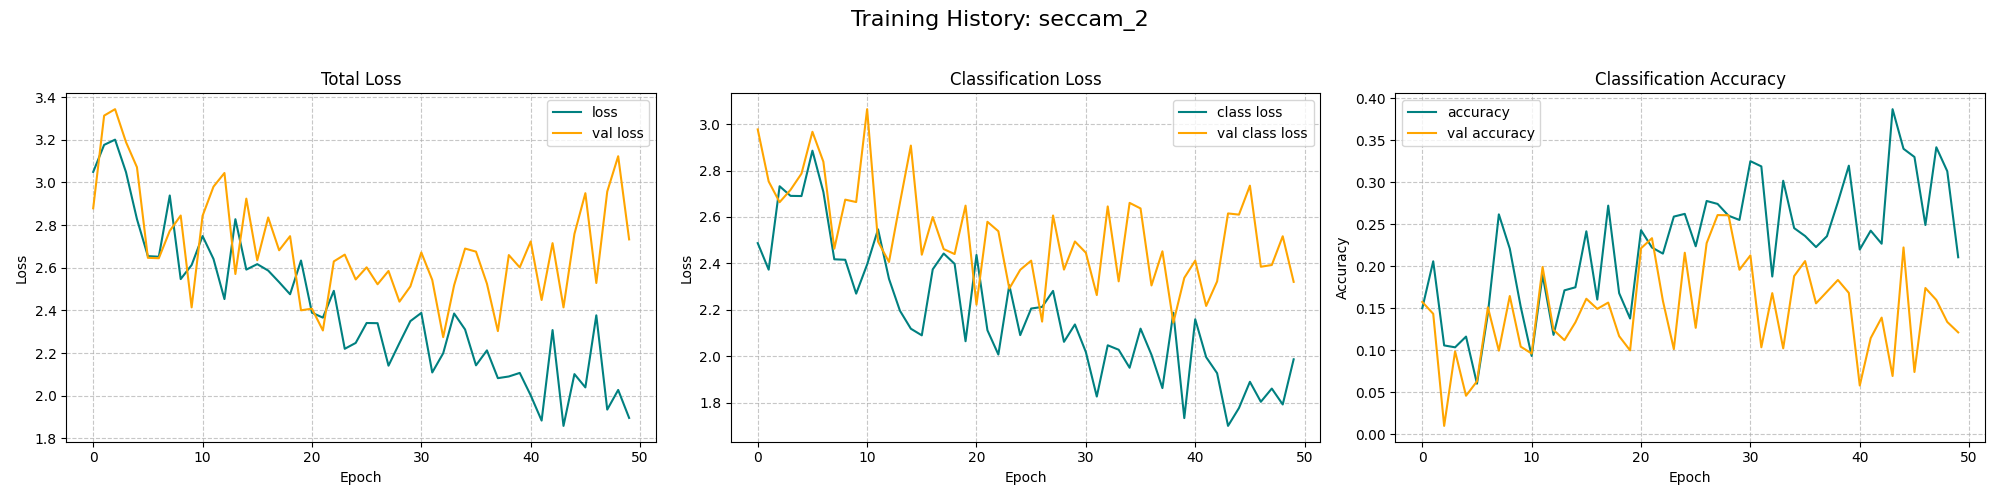
\includegraphics[width=\textwidth]{../Files/training_seccam_2.png}
    \caption{Training performance on the second security camera dataset. Accuracy barely improves due to low-quality data and high face similarity.}
    \label{fig:training-seccam-2}
\end{figure}

\subsection{Summary}
The training results highlight the challenges of dataset quality and overfitting:
\begin{itemize}
    \item The webcam dataset model appears overfitted, as indicated by the plateaued loss.
    \item The first security camera dataset yields slightly worse predictions but demonstrates meaningful improvements.
    \item The second security camera dataset struggles to improve accuracy due to low-quality data and high face similarity.
\end{itemize}

\section{System Architecture and Integration}

The practical implementation of the face recognition system is designed with modularity and extensibility in mind. The architecture is composed of several core modules, each responsible for a distinct aspect of the application workflow:
\textbf{Camera Module (\texttt{camera.py}):} Handles real-time video capture and face detection from a camera stream.
\textbf{Model Module (\texttt{model.py}):} Provides face detection and recognition capabilities, including embedding extraction and evaluation.
\textbf{Database Module (\texttt{database.py}):} Manages persistent storage of face embeddings and detection logs, supporting both PostgreSQL and CSV-based backends.
\textbf{Main Application (\texttt{main.py}):} Orchestrates the end-to-end attendance system, integrating camera input, face recognition, and database operations.

\begin{figure}[ht!]
    \centering
    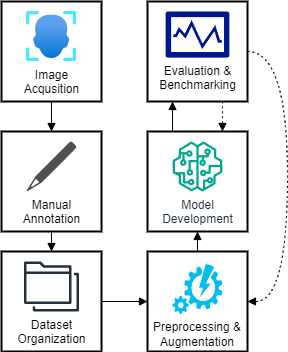
\includegraphics[width=0.7\textwidth]{../Files/codebase_workflow.png}
    \caption{Codebase workflow illustrating the interaction between modules.}
    \label{fig:codebase-workflow}
\end{figure}

\begin{figure}[ht!]
    \centering
    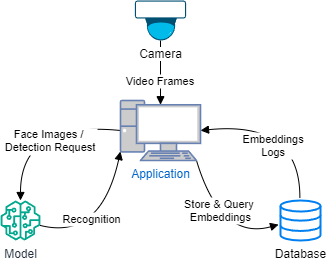
\includegraphics[width=0.7\textwidth]{../Files/system_architecture.png}
    \caption{Modular architecture of the face recognition attendance system.}
    \label{fig:system-architecture}
\end{figure}

\subsection{Camera Module (\texttt{camera.py})}
The \texttt{Camera} class encapsulates the logic for interfacing with a video capture device (e.g., webcam or RTSP stream). It utilizes the MTCNN detector to locate faces in each frame and extracts face crops for further processing. The module provides methods to:
\begin{itemize}
    \item Capture frames from the camera.
    \item Detect faces and return their bounding boxes and cropped images.
    \item Release camera resources when finished.
\end{itemize}

\subsection{Model Module (\texttt{model.py})}
The \texttt{FaceTracker} class is responsible for both face detection and recognition. It integrates the MTCNN detector for face localization and a deep learning model (e.g., EfficientNet or VGG16-based) for generating face embeddings. Key functionalities include:
\begin{itemize}
    \item Detecting faces in input images.
    \item Extracting and normalizing face embeddings for recognition.
    \item Evaluating recognition accuracy on test datasets using cosine similarity.
\end{itemize}

\subsection{Database Module (\texttt{database.py})}
The \texttt{FaceDatabase} class abstracts the storage and retrieval of face embeddings and detection logs. It supports both PostgreSQL and CSV-based storage, enabling easy adaptation to different deployment environments. Its main responsibilities are:
\begin{itemize}
    \item Adding new face embeddings to the database.
    \item Retrieving all stored embeddings for comparison.
    \item Logging detection events with timestamps and labels.
\end{itemize}

\subsection{Main Application (\texttt{main.py})}
The \texttt{AttendanceApp} class serves as the entry point for the real-time face recognition attendance system. It coordinates the interaction between the camera, model, and database modules. The main workflow is as follows:
\begin{enumerate}
    \item \textbf{Frame Acquisition:} Continuously captures frames from the camera.
    \item \textbf{Face Detection and Recognition:} For each detected face, extracts embeddings and compares them to the database.
    \item \textbf{Identification and Logging:} Assigns an identity (existing or new), draws bounding boxes and labels on the frame, and logs the detection event.
    \item \textbf{User Interface:} Displays the processed video stream with real-time annotations.
\end{enumerate}

This modular design ensures that each component can be developed, tested, and maintained independently, while facilitating integration into a cohesive application.


